\chapter{Introduction}\label{chap_introduction}

\todo{comment from Lucia:I really don't like this sentence.
Maybe something along these lines: "Every human cell carries the genetic information needed to accomplish specific biological program. Such information is included in two sets of 23 chromosomes, with each set containing approximately 3 billion DNA bases."

Every normal cell of every human being contains two sets of 23 chromosomes, with the chromosomes in each set holding approximately three billion chained nucleotides of DNA. 

This DNA contains the instructions that the cell uses to code for the proteins that ultimately specify the behavior of the cell, and in aggregate affect the characteristics of the individual to whom the cell belongs. 

The differences between the DNA of the cells in two individuals can explain differences in their physical characteristics, their risk of disease, and their population origin and evolutionary history. 

If one of the cells is cancerous, the differences in the DNA of two cells in one individual can explain the origin of their disease and potentially predict effective treatments.

 through the proteins they code for and the programs of gene expression they regulate}

The aim of the field of \emph{genomics} is to characterize the structure and function of the DNA of an organism or population of organisms, with the ultimate goal of understanding how the sequences of nucleotides that make up the genome affect phenotypes and reveal evolutionary history. To do so, it is necessary to identify and understand the differences between the DNA from two samples, whether the samples come from two different individuals or two different tissues from the same individual. Given that each sample can contain DNA from multiple cells, and each cell in a human sample contains approximately 3 billion DNA bases packaged into two sets of 23 chromosomes, this is difficult and complex undertaking.

If, as is the case for humans, the species has been widely studied, a \emph{reference genome} is often used in place of one of the samples. This allows variations between individuals to be described as variations between the sample and the reference. Experiments of this type are known as \emph{resequencing} experiments. Assuming that a reference is used, or that the samples come from an individual or individuals from the same or closely related species, the majority of the DNA sequence will be the same between the two samples. In that case, variants can be categorized into one of several forms. The first is a difference of a single base of DNA at a particular location within the genome, or a \emph{single nucleotide variant} (SNV). If the variation is shared between many individuals in a population, these are referred to as \emph{single nucleotide polymorphisms} (SNPs). Another type of variation is the insertion or deletion of a small number of base pairs at a particular location, commonly referred to as \emph{indels}. A final category of variants are genomic \emph{structural variations} (SVs). This term describes variations that affect a large number of bases of DNA (in common usage at least 40 base pairs, ranging up to hundreds of megabases or entire chromosomes). SVs can take a variety of forms: strings of DNA can be deleted, inserted, duplicated, inverted, or translocated to a different chromosome. Because they can be large and frequent, SVs account for the majority of the bases that differ among normal human genomes~\cite{Mills:2011p1611, Conrad:2010ja}.

All of these types of variants can alter the function of a genome in different ways. SNVs can change the sequence of the proteins coded for by genes, sometimes altering their function and sometimes rendering them inactive, or they can alter regulatory elements and cause genes to be expressed at differing levels. Indels typically disrupt the function of a gene or regulatory element. SV's can cause a variety of functional changes, ranging from the deletion of exons to the formation of fusion genes such as the famous Brc-Abl Philadelphia chromosome in chronic myelogenous leukemia~\cite{Kurzrock:2003bz}. 

\todo{change this??}
In fact, SVs are very common in some types of cancer, producing extremely rearranged genomes. Because of this, they have particular importance in cancer research, and it is therefore essential to be able to identify them in biological samples, as well as to characterize their functional impact and the mechanisms of their formation. The SVs that arise in cancer genomes have similarities to those that have arisen between different species in evolution (Figure~\ref{cancer_evolution_breakpoints}). For example, the genomes of gibbon species, while still closely related to humans and other apes, have undergone a variety of chromosomal rearrangements and other structural variations when compared to these other species; many more, in fact, than are typical in species with similar levels of divergence. Understanding the evolutionary changes in gibbons, therefore, may shed light on the much faster processes that take place in progenitor cancer cells.

\begin{figure}
\centering
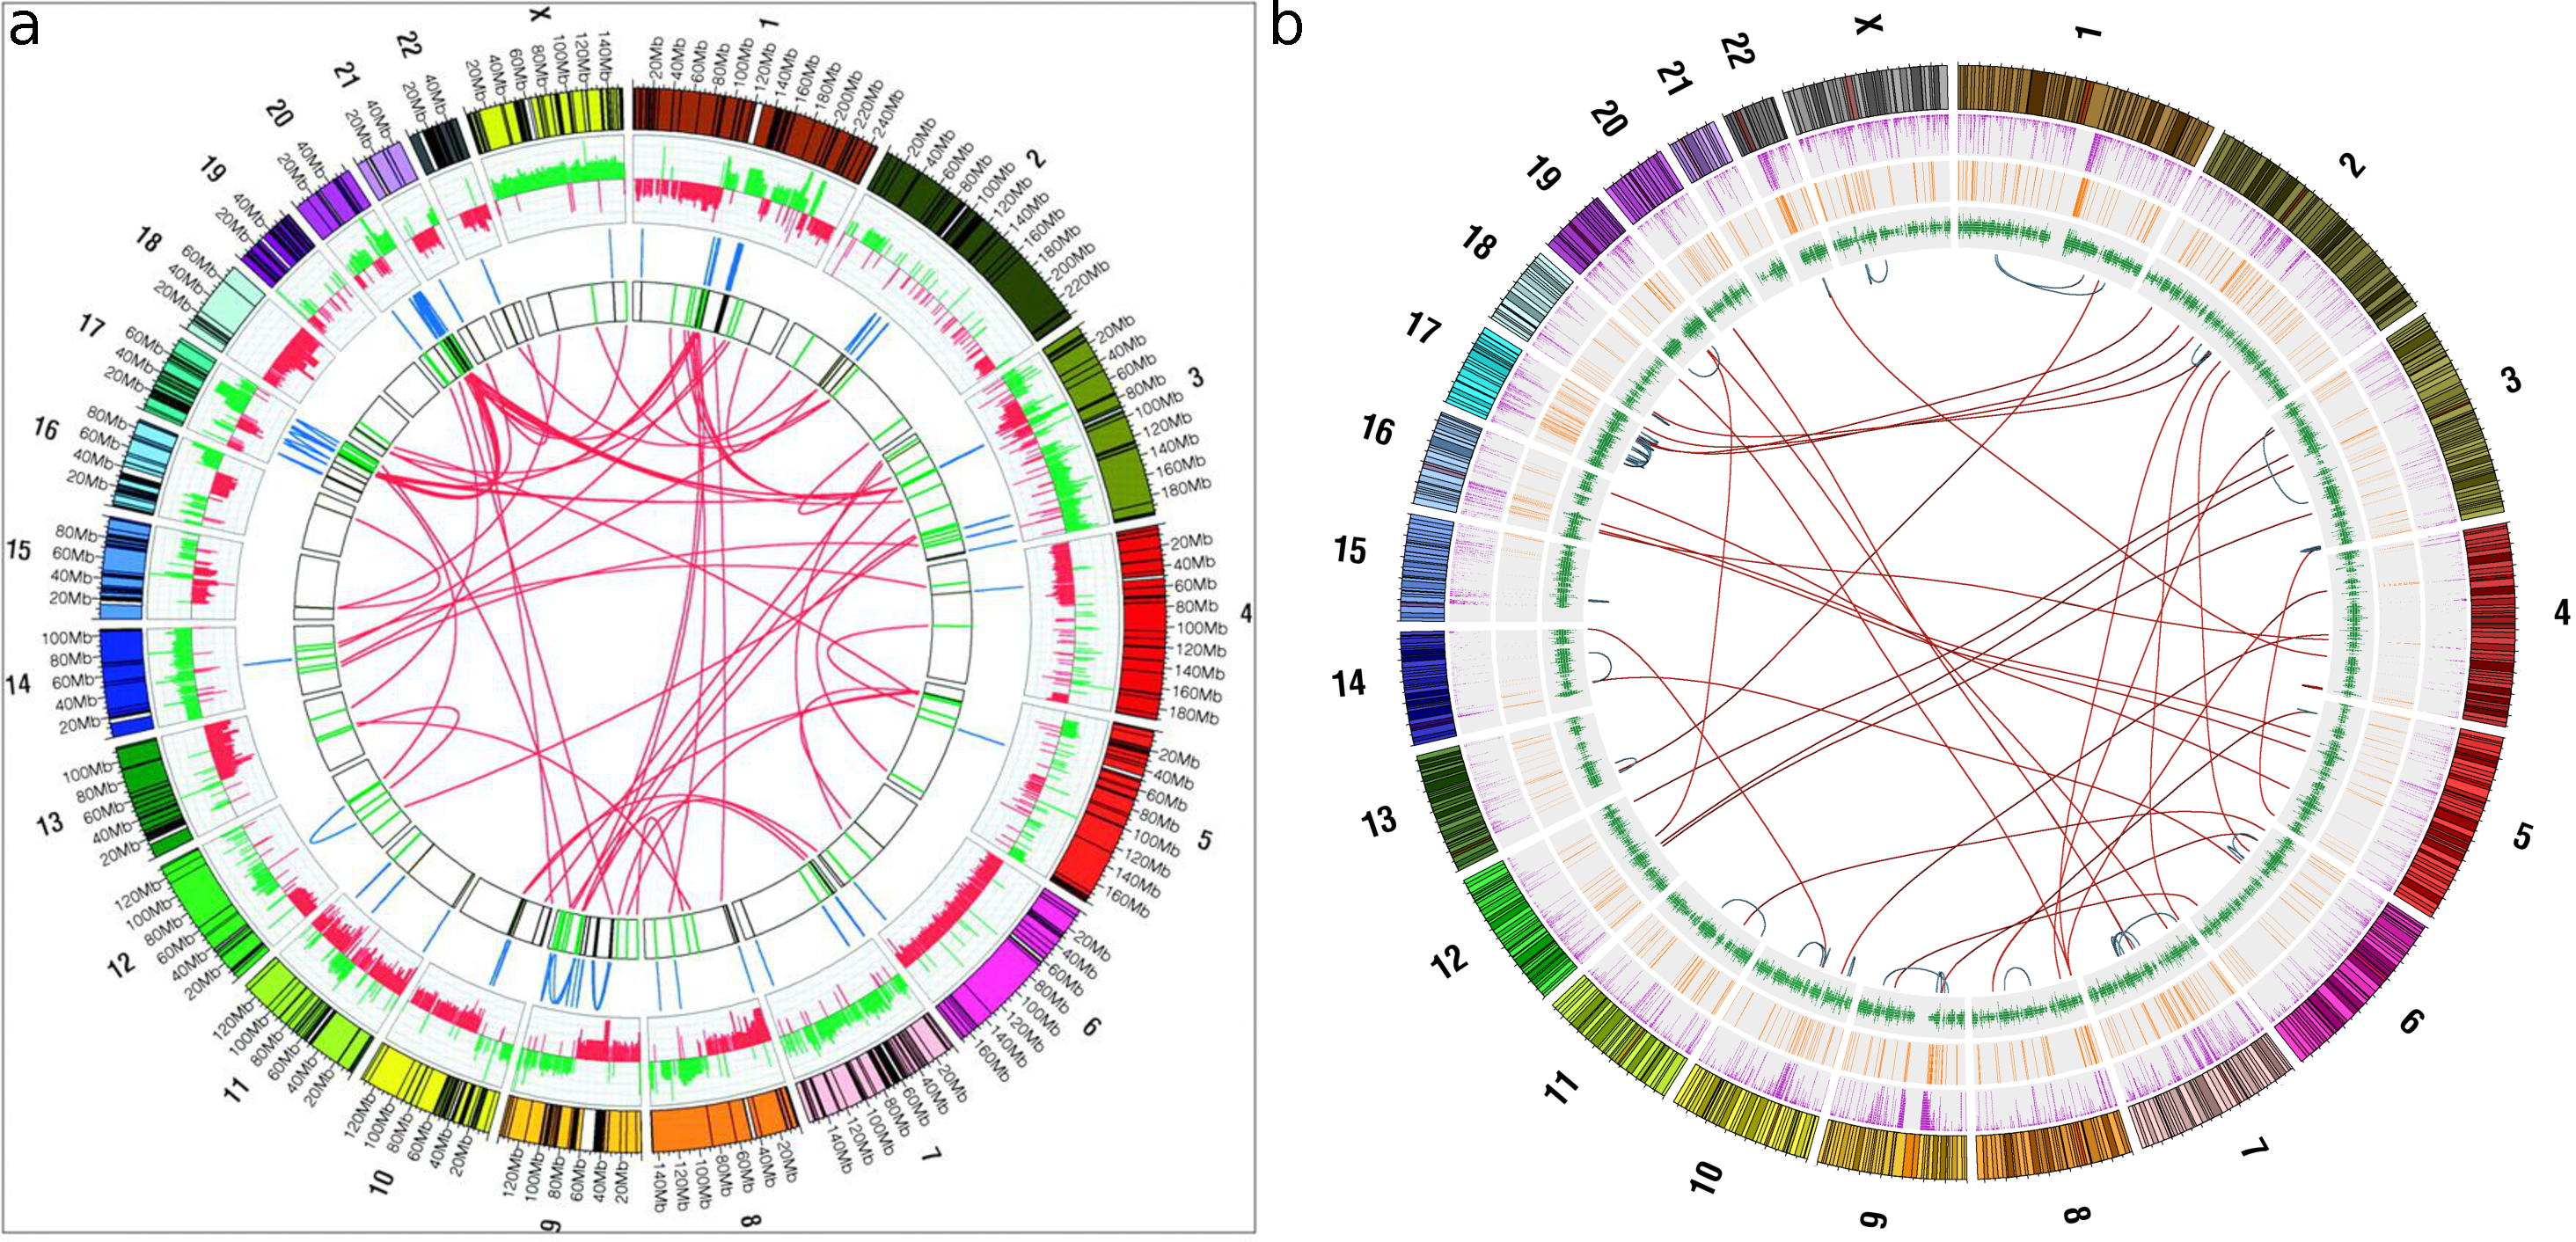
\includegraphics[width=.9\textwidth]{figures/breakpoints_in_cancer_and_evolution.pdf}
\caption[Similarity of genomic breakpoints that occur in cancer and evolution.]{Similarity of genomic breakpoints that occur in cancer and evolution. The regions around the circle represent the human chromosomes. Lines in the centers of the circles show rearrangements between and within chromosomes. A) Somatic rearrangements detected within a breast cancer cell line, adapted from~\cite{Hampton:2009fc}. B) Rearrangements with respect to the human genome sequence present in the gibbon genome, adapted from~\cite{Carbone:2009p1012}.}
\label{cancer_evolution_breakpoints}
\end{figure}

The current technology to detect genomic variations is massively parallel, high-throughput sequencing. This procedure involves amplifying the DNA from a sample and then shearing it into small fragments. The ends of those fragments are then sequenced, producing hundreds of millions or billions of \emph{read pairs} for a sample using current, widely used instruments. The challenge of genomics is then to discover the variants present in the sample using only these short reads. By generating and sequencing enough fragments from a sample (quantified in terms of \emph{coverage}, the average number of reads that cover any one locus in the reference genome), the hope is that it should be possible to capture almost all of the important variants in a given sample. Current practices suggest that 30X average coverage depth is required to achieve accuracy in detecting SNVs. Even with this level of coverage, however, the task is made difficult by errors in the sequencing process, the fact that mammalian genomes are filled with repetitive sequences that make it difficult to ascertain the location in the genome that generated a particular read pair, and the computational challenges of analyzing the volume of data generated.

While SNVs and indels can be characterized relatively well from sequencing data using current algorithmic approaches, the identification of SVs remains challenging. SVs often arise within repetitive regions of the genome, making it difficult to align the reads surrounding them unambiguously to the reference genome. In addition, when the boundaries of an SV (the \emph{breakpoints}) fall within a read sequence, it can be difficult to map that read back to its point of origin in the reference sequence. Although some approaches are based on searching for reads that contain breakpoints, it is often necessary to fall back on other signals present in the read set: the distance between successfully mapped read pairs, which should match the size of the fragments generated in the sequencing protocol, and the depth of reads that cover individual loci along the genome. Detection of SVs with current high-throughput sequencing technology remains a difficult problem, with limited concordance between available algorithms and high false discovery rates~\cite{Mills:2011p1611}.

While current approaches struggle with accuracy, they also often fail to consider speed and scalability. A 30X coverage data set for an individual sample, in compressed format with associated quality scores, contains over 100GB of data to analyze. A typical bioinformatic pipeline includes steps to run quality control checks on the raw data; align the reads to the reference genome; perform filtering and recalibration steps after alignment; call SNVs and indels; and finally search for SVs. While a great deal of effort has been put into developing, optimizing, and parallelizing fast methods for alignment and variant calling, SV detection algorithms have not received the same attention, primarily because research in SV detection algorithms has focused on improving accuracy. As large scale sequencing projects like the 1000 Genomes Project and The Cancer Genome Atlas grow, the need for fast and accurate algorithms is becoming more apparent. DNA sequencing is already moving into the clinic, which will only exacerbate this requirement by requiring rapid analysis turnarounds for patients.

One approach to scaling data analysis pipelines is to harness the power of distributed computing using frameworks that tie together clusters of servers. Google's MapReduce~\cite{Dean:2008p277} framework was designed to manage the storage and efficient processing of very large scale data sets across clusters of commodity servers. Hadoop is an open source project of the Apache Foundation which provides an implementation of the MapReduce programming framework as well as a distributed file system (HDFS) for distributing the redundant storage of large data sets across a cluster. Hadoop and MapReduce are rapidly becoming a standard in industrial data mining applications. However, they require the use of a specific programming model, which can make it difficult to design general-purpose algorithms for arbitrary sequencing analysis problems like SV detection. 

This thesis presents several novel techniques for detecting SVs using distributed computing and machine learning, which derive from the development of an algorithmic framework for SV detection methods in MapReduce. In particular, the main contributions are:

\begin{itemize}
 \item The description of an algorithmic framework for solving SV detection problems in Hadoop and MapReduce based on the computation of local features along the genome from paired end mappings (Chapter~\ref{chap_framework}).
 \item The development in this framework of a software package, Cloudbreak, for discovering genomic deletions up to 25,000bp long, and short insertions, which improves accuracy over existing approaches and uses distributed computing to achieve dramatically faster runtimes (Chapter~\ref{chap_cloudbreak_impl} and Chapter~\ref{chap_cloudbreak_eval}).
 \item An evaluation of the strengths and weaknesses of Cloudbreak, as compared to several other popular SV detection tools, when tested on several real and simulated data sets (Chapter~\ref{chap_cloudbreak_eval}).
 \item An exploration of the use of local features as described in Chapter~\ref{chap_framework} to reformulate SV detection as a sequence labeling problem, and the corresponding implementation and evaluation of a conditional random field model to create a novel method for integrating different signals of structural variations (Chapter~\ref{chap_crf}).
\end{itemize}

In separate work not related to the algorithmic developments listed above, we also present the results of data analysis projects which examined the SVs that have massively rearranged the genome of the gibbon in an evolutionary time frame. This has led to the additional contribution of:

\begin{itemize}
 \item Identification of sets of genomic features that are enriched near the breakpoints of the structural variations are present between gibbons and humans. These include segmental duplications and some families of transposable elements, as well as evolutionarily shared transcription factor binding sites. This analysis enhances our understanding of gibbon genome rearrangements. (Chapter~\ref{chap_breakpoint_analysis}).
\end{itemize}

A preliminary version of parts of this work was peer-reviewed and accepted for oral presentation at the Third Annual RECOMB Satellite Workshop On Massively Parallel Sequencing (RECOMB-seq). A preliminary breakpoint analysis was published in~\cite{Capozzi:2012bb}. Throughout this document, I have tried to explicitly identify any work that was carried out by my collaborators.
